\documentclass[11pt,a4paper]{ltjsarticle}
\usepackage{luatexja-fontspec}
\usepackage{geometry}
\usepackage{booktabs}
\usepackage{array}
\usepackage{enumitem}
\usepackage{graphicx}
\usepackage{amsmath}
\usepackage{fancyhdr}
\usepackage{xcolor}
\usepackage{hyperref}

\geometry{margin=24mm}
\setmainjfont[BoldFont=Hiragino Kaku Gothic ProN]{Hiragino Mincho ProN}
\setsansjfont{Hiragino Kaku Gothic ProN}
\setmonofont{Menlo}
\hypersetup{colorlinks=true, linkcolor=blue!55!black, urlcolor=blue!55!black}

\pagestyle{fancy}
\fancyhf{}
\lhead{研究進捗報告}
\rhead{2026 年 8 月 9 日}
\cfoot{\thepage}
\renewcommand{\headrulewidth}{0.2pt}

\newcommand{\rk}{\textrm{Recall@}K}
\setlist{nosep}

\begin{document}

\begin{center}
{\sffamily\large 物理モデルの自動構築：期待した特徴量はなぜ効かなかったのか}
\end{center}
\vspace{0.3em}
\hfill 作成者：M2\ 一洋
\vspace{0.8em}

%======================================================================
\section{前回ゼミレビュー}
%======================================================================
\textbf{研究の目的}：科学文献から数式を集めておき、「どんな物理モデルを作りたいか」（説明文と入出力変数）を入力すると、そのモデルを構成するのに必要な\textbf{数式の集合}を提示する。

本手法は 2 段構えである。\textbf{第 1 段}では、データベースの全 11{,}146 式に、説明文と式まわりの文章がどれだけ似ているか（\textbf{文章類似度}）と、指定された入出力変数と式の変数がどれだけ重なるか（\textbf{変数の一致度}）を 7 対 3 の重みで足した点数を付け、上位の何件かを候補として絞り込む。\textbf{第 2 段}では、その候補だけを対象に、10 個の特徴量を多層パーセプトロン（MLP）で学習して並べ直す。候補件数は精度の主要比較では 50 件、その後の実験では 200 件を用いている。

前回は、古典的情報検索手法（baseline）から本手法（reranker-10S）への $\rk$（正解式数 $K$ に合わせ、上位 $K$ 件に入った正解式の割合）の向上 $+0.222$（設定 A：オリジナル＋文献横断＋DAE、1{,}823 件）を報告した。あわせて全 10 特徴量を 1 つずつ評価し、精度を上げるのは\textbf{変数の重なりを測る特徴量}に限られ、\textbf{話題の近さを測る特徴量（意味の近さ・分野の一致）はどの形でも効かない}ことを示した。

%======================================================================
\section{今回の進捗}
%======================================================================
これに対し\textbf{加藤先生から「性能向上手法として期待していたことと結果との関連、およびその原因の考察が要る。正解・不正解のケースを見て分析すること。意味の近さが効かないのは、TF-IDF から SVD で計算したベクトルがケース間であまり違わないためではないか」とのご指摘}をいただいた。本報告では、この原因を実験で調べた。

\begin{enumerate}[leftmargin=1.8em]
  \item \textbf{ベクトルの差が小さいという仮説は成り立たなかった}：ケースどうしのベクトルは十分に離れていた。意味の近さは、全データベース 11{,}146 式の中から正解式を選び出す力も十分に持っていた。
  \item \textbf{原因は、候補を絞った後では話題の情報が要らなくなることであった}：話題の近さは全データベースから候補を絞るときには強く効くが、候補に絞った後では正解式と不正解式をほとんど区別できない。
  \item \textbf{誤りがどこで生じるかは、候補件数で入れ替わる}：候補 50 件では上位 $K$ 件に入らなかった正解式の 61.8\% が第 1 段の候補に入っていなかったが、候補 200 件では 28.4\% に下がり、残りは並べ替えの誤りになる。
  \item \textbf{並べ替えの誤りは、話題の近さを強めても直らない}：候補 200 件では、話題の近さを強めるとかえって順位が悪くなる側にある。
  \item \textbf{訓練し直さずに特徴量の重要度を測る方法を実装し、分野の一致がケースによっては精度を下げていることを見つけた}：全体平均では効果がないように見えるが、正しく働くケースと逆に働くケースが打ち消し合っていた。
\end{enumerate}

%======================================================================
\section{実験 1：意味の近さはどこで効かなくなるか}\label{sec:exp1}
%======================================================================
\textbf{方法}：モデルを訓練せず、データと第 1 段の性質だけから調べた。(a) ケースどうしのベクトルがどれだけ離れているかを、無作為に選んだ 20 万組のコサイン類似度で測った。(b) 1 つの特徴量だけで正解式を不正解式より上に並べられる割合（AUC）を、\textbf{全データベース 11{,}146 式を相手にした場合}と\textbf{第 1 段が選んだ候補の中}で測った。AUC は 0.5 が識別力なし、1.0 が完全な分離を表す。

\textbf{結果}（図~\ref{fig:diag}・表~\ref{tab:auc}）：
\begin{itemize}[leftmargin=1.5em]
  \item \textbf{仮説は成り立たなかった}：ケースどうしのコサイン類似度は中央値 $0.218$ で、$0.5$ を超える組は 5.4\% にとどまる（図~\ref{fig:diag}(a)）。同じ内容のケースの組（説明文を書き換えただけの組）が $0.94$ 以上に集まることと比べると、無関係な水準である。さらに意味の近さ 1 つで、全データベースから正解式を選び出す AUC は $0.950$ に達する。ベクトルの差が失われていれば、この分離は起こらない。
  \item \textbf{候補を絞った後で効かなくなる}：意味の近さの AUC は全データベースの $0.950$ から、候補 50 件で $0.594$、候補 200 件でも $0.718$ に落ちる。これに対し変数の一致度は $0.999$ から $0.947$／$0.977$ を保ち、式の特化度は候補の中で $0.965$／$0.984$ と最も高い（表~\ref{tab:auc}、図~\ref{fig:diag}(b)）。
  \item \textbf{候補には初めから話題の近い式が集まっている}：第 1 段は文章類似度を重み 7 で使うので、候補に残る不正解式は正解式と話題がそろっている。話題の近さは絞り込みには効くが、絞り込んだ後の選別には使えない。
\end{itemize}

\begin{table}[h]\centering
\small
\caption{1 つの特徴量だけで正解式を不正解式より上に並べられる割合（AUC、1{,}823 ケースの平均$\pm$標準誤差）。式の特化度は候補の中でのみ測った。}
\label{tab:auc}
\begin{tabular}{lccc}
\toprule
特徴量 & 全データベース & 候補 50 件の中 & 候補 200 件の中 \\
\midrule
変数の一致度 & $0.999 \pm 0.000$ & $0.947 \pm 0.002$ & $0.977 \pm 0.001$ \\
式の特化度 & — & $0.965 \pm 0.001$ & $0.984 \pm 0.000$ \\
意味の近さ & $0.950 \pm 0.003$ & $0.594 \pm 0.006$ & $0.718 \pm 0.006$ \\
文章類似度 & $0.913 \pm 0.003$ & $0.437 \pm 0.007$ & $0.572 \pm 0.007$ \\
\bottomrule
\end{tabular}
\end{table}

\begin{figure}[h]\centering
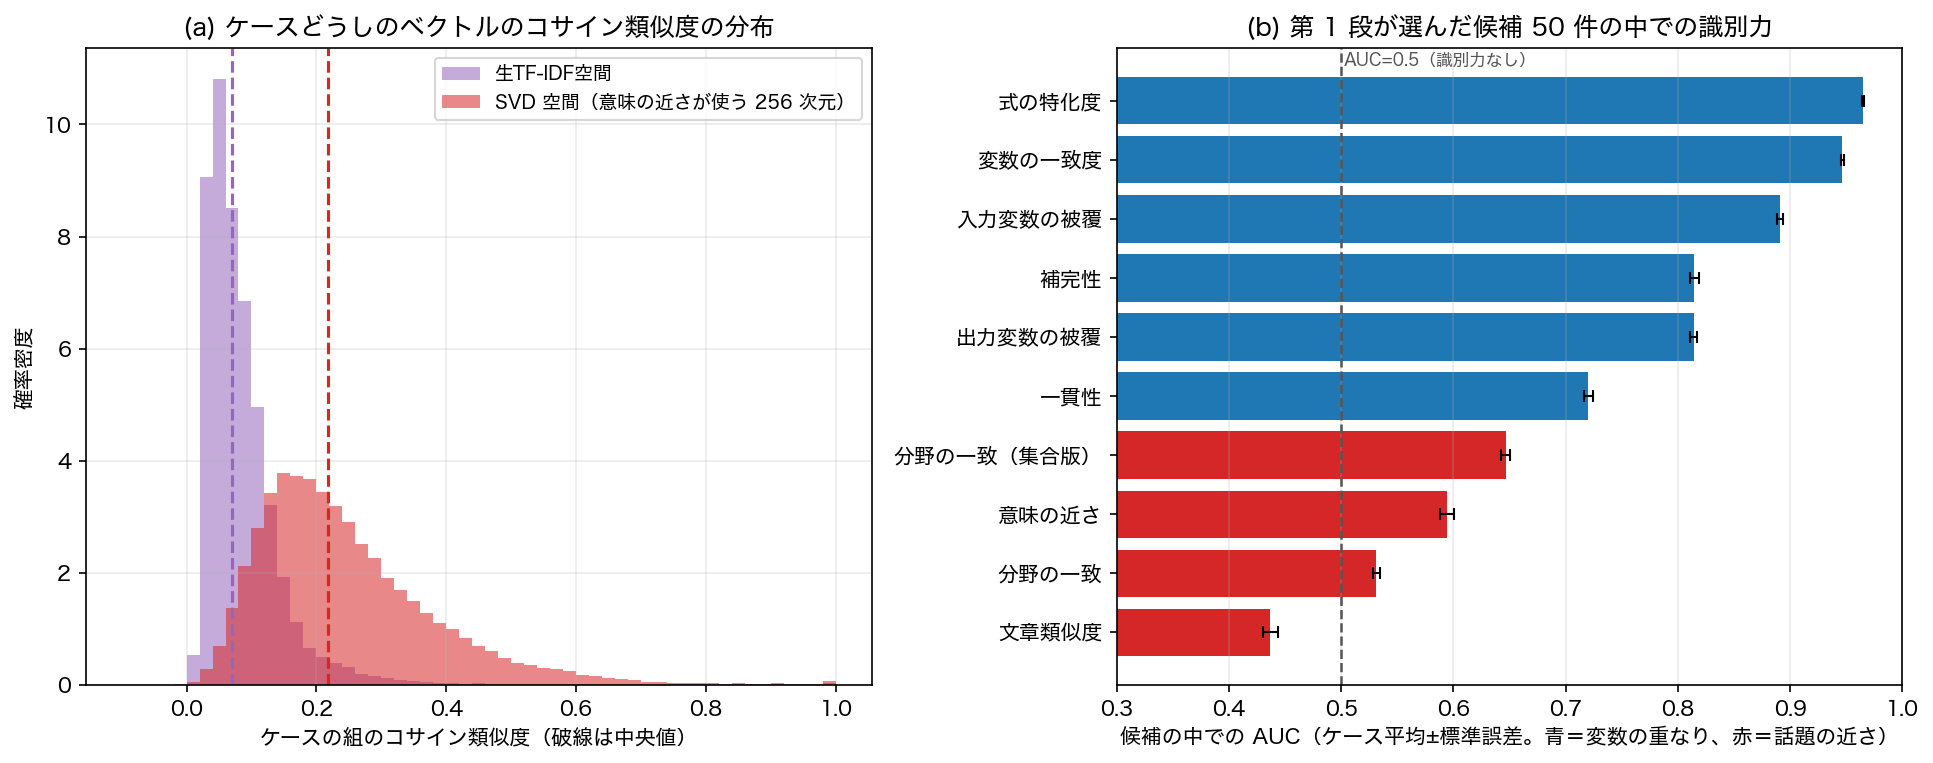
\includegraphics[width=0.90\linewidth]{figures/fig_topic_diagnosis.png}
\caption{(a) ケースどうしのベクトルのコサイン類似度の分布（無作為に選んだ 20 万組、破線は中央値）。(b) 候補 50 件の中で正解式を不正解式より上に並べられる割合（1{,}823 ケースの平均、誤差棒は標準誤差。青は変数の重なりを測る特徴量、赤は話題の近さを測る特徴量）。}
\label{fig:diag}
\end{figure}

%======================================================================
\section{実験 2：正解・不正解のケースを見る}\label{sec:exp2}
%======================================================================
\textbf{方法}：本手法を乱数 1 通り（seed 42）で訓練し、テストの 423 ケースを、正解式をすべて上位 $K$ 件にそろえられたケースと、そろえられなかったケースに分けた。上位 $K$ 件に入らなかった正解式ごとに、\textbf{第 1 段で候補に入らなかったもの}と、\textbf{候補には入ったが上位 $K$ 件から漏れたもの}を区別した。候補 50 件と 200 件で同じ手順を繰り返した。

\textbf{結果}：
\begin{itemize}[leftmargin=1.5em]
  \item \textbf{誤りの内訳は候補件数で入れ替わる}：候補 50 件では、上位 $K$ 件に入らなかった正解式 435 本のうち 269 本（61.8\%）が第 1 段で候補に入らなかった。候補 200 件にすると $\rk$ は $0.791\to0.807$ に上がり、入らなかった正解式は 373 本に減る。その内訳は第 1 段が 106 本（28.4\%）、並べ替えが 267 本（71.6\%）と逆転する。設定 B（DAE のみ 1{,}000 件）でも、候補を 50 件から 200 件に広げると $\rk$ は $0.689\to0.724$ に上がる（乱数 10 通り）。
  \item \textbf{そろえられないのは規模の大きいケースである}：そろえられなかったケースの正解式数は平均 $5.34$（そろえられたケースは $2.13$）、入力変数数は $17.8$（同 $10.8$）であった。候補 200 件でも傾向は同じである。
  \item \textbf{並べ替えの誤りは話題の近さを強めても直らない}：上位 $K$ 件に入らなかった正解式と、その代わりに上位へ入った誤りの式を組にして意味の近さを比べると、正解式のほうが大きい組は候補 50 件で $0.516$、候補 200 件で $0.421$ であった。$0.5$ なら両者は区別が付かず、$0.5$ を下回れば強めるとかえって順位が悪くなる。
  \item \textbf{誤りの型は 2 つに分けられた}。
  \begin{itemize}[leftmargin=1.2em]
    \item \textbf{別の文献にある数学的に同じ式を選ぶ}：回分発酵のケース（入力：時間 $t$・比増殖速度 $\mu$／出力：菌体濃度 $X$）で、正解は出典文献の $dX/dt = \mu X$ だが、\textbf{別の文献}の $(1/X)\,dX/dt = \mu$ と $dX/dt = \mu \cdot X$ が上位に来た。3 式とも変数は同じで変数側の特徴量では区別できず、意味の近さは誤りのほう（$0.72$ と $0.584$）が正解（$0.369$）より大きい。
    \item \textbf{式の向きを表せない}：非等温 CSTR の線形化応答のケース（出力：濃度偏差 $C_A'$）で、正解 $dC_A'/dt = a_{11}C_A' + a_{12}T' + \cdots$ と誤り $dT'/dt = a_{21}C_A' + a_{22}T' + \cdots$ が全特徴量でほぼ同値になった。両者の違いは\textbf{どの変数を左辺で決める式か}であり、変数の集合しか見ない現在の特徴量では表せない。
  \end{itemize}
  \item \textbf{上限を決めているのは候補件数である}：正解式が候補に入る割合（被覆率）は第 2 段の $\rk$ の上限になる。現行の重みでは候補 50 件で $0.920$、200 件で $0.977$ である。変数の一致度だけで絞ると 50 件で $0.961$ まで上がるが、200 件では $0.991$ で差は小さい。候補を広げれば重み付けの調整はほとんど要らない。
\end{itemize}

%======================================================================
\section{実験 3：モデルが実際に使っている特徴量を、訓練し直さずに測る}\label{sec:exp3}
%======================================================================
\textbf{方法}：これまで「どの特徴量が効くか」は、特徴量を 1 つずつ足したモデルを訓練し直して比べる方法で調べてきた（前回報告）。今回はこれとは別に、\textbf{訓練済みの最良モデルを 1 つだけ用意し、ある特徴量の値をケース内でシャッフルして $\rk$ がどれだけ下がるかを測る}方法（順列特徴量重要度）を実装した。訓練し直さないので、モデルが実際にその特徴量へどれだけ頼っているかを直接測れる。設定 A・乱数 10 通り・各特徴量あたり 20 回のシャッフルで実施し、さらにケースごとに分解した（727 ケース）。

\textbf{結果}（表~\ref{tab:pfi}）：
\begin{itemize}[leftmargin=1.5em]
  \item \textbf{訓練し直す方法と同じ結論に至った}：変数の重なりを測る 6 特徴量をまとめてシャッフルすると $\rk$ は $0.743$ から $0.065$ に下がる（$p<0.001$）。話題の近さを測る 4 特徴量をまとめてシャッフルしても $+0.006$（$p=0.10$）で、ほとんど変わらない。式の特化度 1 つで $+0.617$ を占める。
  \item \textbf{分野の一致は、ケースによっては精度を下げていた}：全体平均は $-0.000$（$p=0.91$）で効果がないように見えるが、ケースを分けると、この特徴量が正解式を上位に寄せているケース（1{,}169 件）では平均 $+0.012$ の低下、逆向きに働いているケース（414 件）では $-0.034$、すなわち\textbf{シャッフルするとかえって精度が上がる}。両者が打ち消し合って平均がゼロになっていた（$p = 1.3\times10^{-8}$）。補完性と一貫性にはこれは無く、どちらの向きのケースでも低下は正である。
\end{itemize}

\begin{table}[h]\centering
\small
\caption{集合特徴量をケース内でシャッフルしたときの $\rk$ の低下（727 ケース、平均$\pm$標準誤差）。その特徴量が正解式を上位に寄せているケースと、逆向きに働いているケースに分けた。低下が負の値は、シャッフルするとかえって精度が上がることを意味する。}
\label{tab:pfi}
\begin{tabular}{lcc}
\toprule
特徴量 & 正しい向きのケース & 逆向きのケース \\
\midrule
補完性 & $+0.026 \pm 0.003$ & $+0.013 \pm 0.013$ \\
一貫性 & $+0.024 \pm 0.003$ & $+0.047 \pm 0.008$ \\
分野の一致 & $+0.012 \pm 0.002$ & $\mathbf{-0.034 \pm 0.006}$ \\
\bottomrule
\end{tabular}
\end{table}

%======================================================================
\section{まとめと今後の課題}
%======================================================================
\textbf{今回}：意味の近さが効かない原因が、ご指摘のベクトルの計算方法ではなく、\textbf{第 1 段で候補を絞った後には話題の情報が要らなくなること}にあることを示した。全データベースを相手にすれば意味の近さだけで AUC $0.950$ に達するが、候補の中では $0.594$／$0.718$ にとどまる。あわせて正解・不正解のケースを分けて調べ、誤りの所在が候補件数で入れ替わること、残る並べ替えの誤りは話題の近さを強めても直らないこと、誤りが「別の文献の同じ式」と「式の向きの区別が付かない」の 2 型であることを示した。さらに、訓練し直さずに特徴量の重要度を測る方法を実装し、分野の一致がケースによっては精度を下げていることを見つけた。

\textbf{今後の課題}：
\begin{itemize}[leftmargin=1.5em]
  \item 精度の主要比較と特徴量の評価を候補 200 件でも測り直し、話題の近さが効かないという結論が候補件数に依存しないことを確かめる。
  \item 候補を広げても残る並べ替えの誤りに対し、式の向き（どの変数を決める式か）を表す特徴量を設計する。
  \item 分野の一致は逆向きに働くケースで精度を下げているので、この特徴量を外した場合の精度を測る。
\end{itemize}

\end{document}
